\subsection{part a}

We used get\_fog and opt\_app to find first order time delay transfer function (FOTF).
\begin{itemize}
    \item frequency
    $$
    G(s) =  e^{-1.45*s} \dfrac{0.375}{0.9587s + 1}
    $$
    \item transfer function
    $$
    G(s) =  e^{-1.39*s} \dfrac{0.375}{0.9428s + 1}
    $$
    \item optimum
    $$
    G(s) =  e^{-1.38*s} \dfrac{0.383}{s + 1.021}
    $$
\end{itemize}
\begin{figure}[H]
    \caption{system and FOTD step responde}
    \centering
    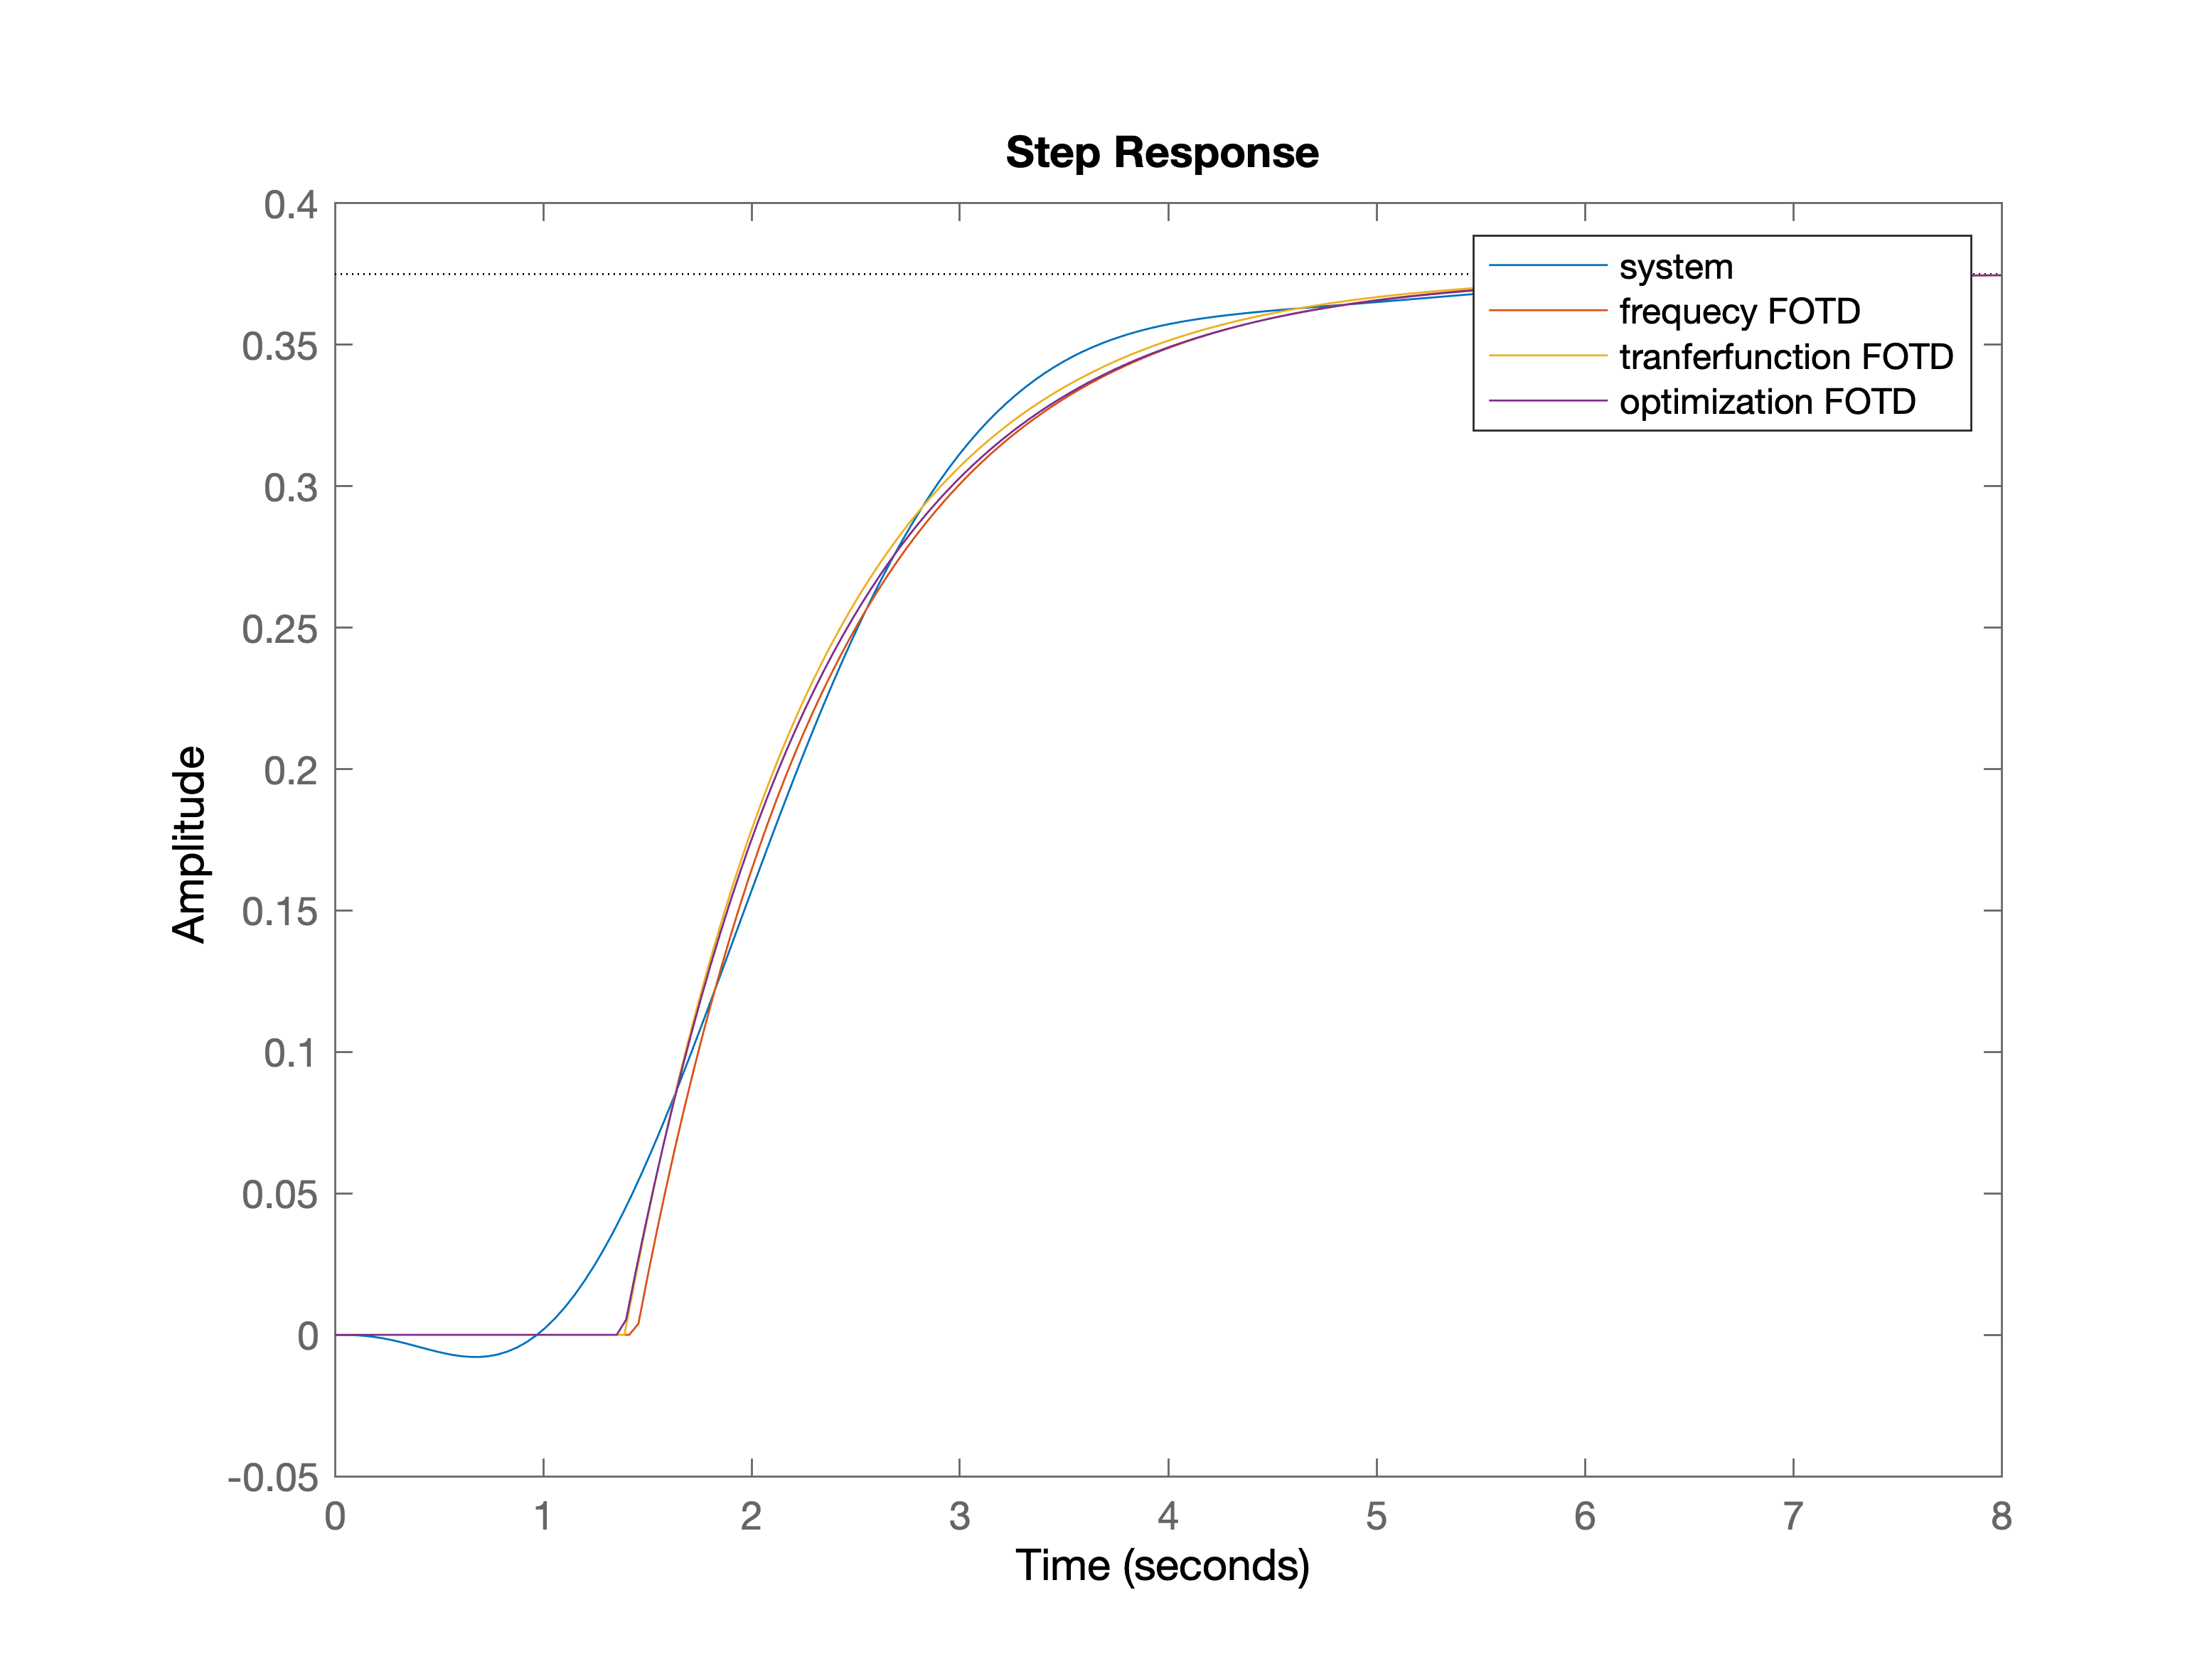
\includegraphics[width=12cm]{../Figure/Q1/a/FOTD.png}
\end{figure}
I used below cost function to see witch one fits better.
$$
\text{Cost} = \int_{0}^{8} \vert G(t) - G'(t)\vert dt,\qquad \text{$G'$ is FOTD transfer function}
$$
\begin{itemize}
    \item frequency
    
    Cost = 1.5949
    \item transfer function
    
    Cost = 1.3208
    \item optimum
    
    Cost = 1.0345
\end{itemize}